
\QCMautoevaluation{Pour chaque question, plusieurs réponses sont
  proposées.  Déterminer celles qui sont correctes.}

\begin{QCM}
  \begin{GroupeQCM} 
  
    \begin{exercice}
      L'équation $2x – 6 = 2(– 2 + x)$...
      \begin{ChoixQCM}{4}
      \item admet 0 pour solution
      \item admet 2 pour solution
      \item a les mêmes solutions que $0x = 2$
      \item n'a pas de solution
      \end{ChoixQCM}
\begin{corrige}
     \reponseQCM{cd}
   \end{corrige}
    \end{exercice}
    
      \begin{exercice}
      « Le double de la somme d'un nombre et de 3 est égal à la moitié de ce nombre, augmentée de 5 »
      \begin{ChoixQCM}{4}
      \item $\dfrac{x}{2} + 3 = 2x + 5$
      \item $2x + 3 = \dfrac{x}{2} + 5$
      \item $2(x + 3) = \dfrac{x+5}{2}$
      \item ce nombre n'a pas d'écriture décimale
      \end{ChoixQCM}
\begin{corrige}
     \reponseQCM{b}
   \end{corrige}
    \end{exercice}
    
      \begin{exercice}
     $4x + 3 < 9$ donc...
   \begin{ChoixQCM}{4}
      \item $4x > 9 – 3$
      \item $\dfrac{4x+3}{9}< 1$
      \item $x$ peut être égal à 10
      \item $x < 1,5$
      \end{ChoixQCM}
\begin{corrige}
     \reponseQCM{bd} % ici deux réponses justes
   \end{corrige}
    \end{exercice}
    
      \begin{exercice}
     L'ensemble des nombres strictement supérieurs à 3 est représenté par...
      \begin{ChoixQCM}{4}
      \item 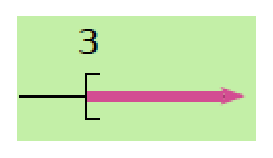
\includegraphics[scale=0.5]{I4}
      \item 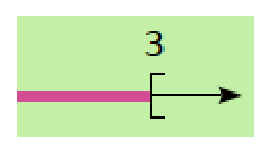
\includegraphics[scale=0.5]{I5}
      \item \includegraphics[scale=0.5]{I6}
      \item 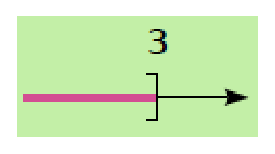
\includegraphics[scale=0.5]{I7}
      \end{ChoixQCM}
\begin{corrige}
     \reponseQCM{c}
   \end{corrige}
    \end{exercice}
    
      \begin{exercice}
    L'inéquation qui a pour solutions tous les nombres  inférieurs ou égaux à $− 2$  est...
      \begin{ChoixQCM}{4}
      \item $3x < − 6$
      \item $x+2\geq 4x+8$
      \item $-5x\leq 10$
      \item $8\geq x+10$
      \end{ChoixQCM}
\begin{corrige}
     \reponseQCM{bd} % ici deux réponses justes
   \end{corrige}
    \end{exercice}
    
      \begin{exercice}
      L'inéquation $2x + 5 \leq 2x + 6$...
      \begin{ChoixQCM}{4}
      \item admet tout nombre positif comme solution
      \item a une infinité de solutions
      \item admet 7 comme solution
      \item n'a pas de solution
      \end{ChoixQCM}
\begin{corrige}
     \reponseQCM{abc} 
   \end{corrige}
    \end{exercice}
   


\end{GroupeQCM}
\end{QCM}

  